\chapter{Future Colliders}
\label{chapter:colliders}

\epigraph{Progress is not a straight line.}{An Wang}

In the post-LHC era, particle physics is at somewhat of an impasse. \acrfull{SM} has held up to most experiments and observation, and its predictive power is now exhausted. There are tantalising hints at a theory beyond the Standard Model -- in the form of CP-violation and dark matter -- but as of yet all new ways to probe the \acrshort{SM} for its weaknesses, to see the greater theory behind it, have yielded very little. 

There are many planned investigations to attempt to identify physics \acrlong{BSM} that use the \acrfull{LHC}, or plan to leverage the upgrades for the \acrfull{HL-LHC}. However, now that the Higgs boson has been identified successfully, one of the most fruitful avenues for further research is the construction and operation of a lepton collider at the energy frontier, with sufficient centre-of-mass energy to produce Higgs bosons in large numbers.

This is what motivates the several proposals for future lepton colliders around the world today, that would operate to complement and expand the reach of particle physicists beyond what the \acrshort{LHC} is currently capable of. These proposed lepton colliders are broadly split into two groups: linear colliders and circular colliders. 

Linear colliders use two accelerator arms pointed towards a single interaction point, and in general are capable of high centre-of-mass energies thanks to developments in accelerator technologies. The main candidates for this style of collider are the \acrfull{ILC} and the \acrfull{CLIC}. 

Circular colliders use a similar layout to the \acrshort{LHC}, with a circular accelerator capable of creating collisions at multiple different interaction points around the circumference of the ring, which permits multiple detectors. The downsides of a circular collider are that lighter particles like electrons are more prone to energy losses via synchrotron radiation, limiting the centre-of-mass energies that a circular lepton collider can operate at. However, in exchange they tend to have much higher luminosities, allowing greater numbers of collisions and higher yields of certain processes or channels. The main candidates for circular colliders are the \acrfull{FCC} and the \acrfull{CEPC}. 

These proposed colliders share many of the same motivations, design considerations, features, and challenges, as does the ongoing international effort in research and development to make these colliders a reality.

\section{The physics case for a lepton collider}
With the observation of a Higgs boson with a mass of 125 GeV, based on data from the \acrlong{LHC}, the Standard Model of particle physics is now functionally complete. All of it's major predictions have been observed. This is a testament to it's quality as a theory, where it's predictive power and accuracy is one of the best in all of the sciences.

But despite this, a multitude of observations have shown that the Standard Model cannot be a complete theory of nature. Many phenomena have been observed that the Standard Model cannot predict, or that don't seem to interact with the Standard Model in any way.

In the post-LHC era, particle physicists are now forced to seek answers to three questions that the Standard Model cannot solve:

\begin{itemize}
	\item What is dark matter? Astrophysics observations support the existence of a neutral, weakly-interacting substance that composes around 85\% of all mass in the universe. Yet this substance cannot be explained by any known form of matter, and is completely unprecedented by the Standard Model.
	\item Why is there so little antimatter? The symmetries inherent in the Standard Model predict that the Big Bang would have created an equal quantity of matter and antimatter. Yet the universe today is dominated by matter.
	\item Why does the Higgs field fill space and give mass to elementary particles? The existence of the Higgs field and the coupling of the Higgs boson to other particles can be understood from the Standard Model but their origin or cause is still unexplained.
\end{itemize}

In order to answer these questions, new theories of physics Beyond the Standard Model (\acrshort{BSM}) have been made, and need to be experimentally tested. To do this, particle collider experiments at the energy frontier are needed. The \acrfull{LHC} has already been used extensively in searches for new physics, in the forms of new particles, rare and exotic decays, supersymmetry, and dark matter.

However, the running of a lepton collider at the energy frontier would be complementary to the \acrshort{LHC}'s continuing physics programme -- there are many events or channels that are inaccessible or difficult to examine in one environment that are much simpler or higher precision in the other. In this way, a lepton collider would help to improve and refine measurements already taken at the \acrshort{LHC}, while also allowing physicists to examine new channels and decays that were not accessible to it. A number of processes and their discovery potential can be seen in Table \ref{table:colliders/physics-goals}.

This follows a historical pattern in particle physics -- as the energy frontier advances, hadron colliders are used to discover new physics and new phenomena, followed by lepton colliders to examine these phenomena in higher precision.

\subsection{Higgs physics}
Of specific interest to searches at lepton colliders would be the Higgs boson itself. Many \acrshort{BSM} models predict differences from the Standard Model in the Higgs sector -- such as several Higgs bosons with different masses, composite Higgs, charged Higgs etc. The comparatively `quiet' environment of a lepton collider allows higher precision measurements of the properties of the Higgs boson, placing better constraints on the presence of new physics. In addition, lepton colliders can easily operate at specific thresholds and ``hot spots'' for Higgs production, permitting a much greater number of events yielding Higgs bosons, and thus a greater sample to examine.

% First confirmation of h->bb decays paper: https://atlas.web.cern.ch/Atlas/GROUPS/PHYSICS/CONFNOTES/ATLAS-CONF-2018-036/
Additionally, the most common decay of the Higgs boson, at a branching ratio of 57.7\%, is the $H \rightarrow b \overline{b}$ process. Despite the high branching ratio, the huge \acrshort{QCD} backgrounds in a hadron collider have made this decay incredibly difficult to observe at the LHC -- in fact, the $H \rightarrow b \overline{b}$ decay has only fairly recently been experimentally verified by the \acrshort{ATLAS} experiment. However, in a lepton collider these \acrshort{QCD} backgrounds are significantly smaller, meaning this decay channel is much easier to analyse, opening up a huge number of Higgs events for analysis and examination.

Another highly interesting process uniquely accessible to lepton colliders is the higgstrahulung reaction: $e^+ e^- \rightarrow Zh$. The decay of the Z boson into lepton pairs $e^+ e^-$ or $\mu^+ \mu^-$ allows high precision kinematic measurements of the process without directly measuring the Higgs boson itself. This allows unprecedented measurement of the Higgs mass, while also making measurements of missing energy possible. If the Higgs boson has invisible decays -- such as dark matter particles or other undiscovered particles that don't couple to the \acrshort{SM} -- the higgstrahlung process allows their existence to be identified.

[...] [High precision and model-independent measurement of the total rate of Higgs decay $\Gamma\textsubscript{h}$]

[...] [Top-Higgs Yukawa coupling, which is highly sensitive to new physics, since it's the strongest Higgs coupling]

\subsection{Top physics}
In addition to the Higgs, the top quark is of high interest to possible physics programmes at a future lepton collider. Since it's discovery at Fermilab in 1995, there have been no lepton colliders operating with sufficient energy to produce top quarks -- unlike the charm and bottom quarks, which were studied in further detail in lepton colliders after their discovery in hadron machines. The production threshold for top quarks is 350 GeV, and no lepton colliders capable of this energy have been constructed, meaning that the advantages of a lepton collider have never been utilised to understand the top quark in greater detail. 

The detailed study of top quarks and their properties that would be made possible by a lepton collider would have many benefits, primarily in the precision of the measurements. Similar to the Higgs, low \acrshort{QCD} backgrounds make reconstruction of top quark events easier to reconstruct. The fact that the collision is between elementary particles, rather than a parton-parton collision as in a hadron collider, also permits are more well-defined centre of mass energy, which is not possible in hadron colliders.

Precision measurements of the top quark is an important test of the \acrshort{SM} -- many \acrshort{BSM} models envision their additional particles as partners of the top quark. The upshot of this is that because of this, these theories propose properties of the top quark that diverge from the SM. In-depth and precise analysis of the top quark's properties would place limits on these theories, in turn allowing the development of better theories. 

[...] [$t \overline{t}$ production threshold studies -- these form an idealised QCD system to study, possibly also a $t \overline{t}$ bound state]

\begin{table}[h]
\centering
	\begin{tabular}{ c | c | c }
	\hline \hline
	\textbf{Energy} & \textbf{Reaction} & \textbf{Physics goal} \\ \hline
	 91 GeV & $e^+ e^- \rightarrow Z$ & ultra-precision electroweak \\ \hline
	 160 GeV & $e^+ e^- \rightarrow WW$ & ultra-precision W mass \\ \hline
	 250 GeV & $e^+ e^- \rightarrow Zh$ & precision Higgs coupling \\ \hline
	 350-500 GeV & $e^+ e^- \rightarrow t\overline{t}$ & top quark mass and couplings \\
	   & $e^+ e^- \rightarrow WW$ & precision W coupling \\
	   & $e^+ e^- \rightarrow \nu \overline{\nu} h$ & precision Higgs coupling \\ \hline
	 500 GeV & $e^+ e^- \rightarrow f \overline{f}$ & precision search for $Z^\prime$ \\
	   & $e^+ e^- \rightarrow t \overline{t}h$ & Higgs coupling to top \\
	   & $e^+ e^- \rightarrow Zhh$ & Higgs self-coupling \\
	   & $e^+ e^- \rightarrow \widetilde{\chi} \widetilde{\chi}$ & search for supersymmetry \\
	   & $e^+ e^- \rightarrow AH, H^+, H^-$ & search for extended Higgs states \\ \hline
	 700-1000 GeV & $e^+ e^- \rightarrow \nu \overline{\nu} hh$ & Higgs self-coupling \\
	   & $e^+ e^- \rightarrow \nu \overline{\nu} VV$ & composite Higgs sector \\
	   & $e^+ e^- \rightarrow  \nu \overline{\nu} t \overline{t}$ & composite Higgs and top \\
	   & $e^+ e^- \rightarrow \tilde{t} \tilde{t}^*$ & search for supersymmetry \\ \hline
	\end{tabular}
	\caption{Physics processes of interest at lepton colliders up to 1 TeV.}
	\label{table:colliders/physics-goals}
\end{table}

\section{The International Linear Collider}
The \acrfull{ILC} is a proposed high-luminosity linear electron-positron collider based upon 1.3 GHz superconducting radio frequency (\acrshort{SCRF}) accelerating technology. The ILC would have a centre of mass energy $\sqrt{s}$ of 250 GeV, upgradable to 500 GeV and then to 1 TeV at a later date. The total footprint of the complex would be 31km in length, with the arms using magnets with an accelerating gradient of 31.5 MVm\textsuperscript{-1} in metre-long superconducting nine-cell niobium cavities operating at 2K.

There were a number of proposed sites for the \acrshort{ILC}, including \acrshort{CERN} in Geneva, \acrshort{DESY} in Hamburg, and \acrshort{JINR} near Moscow. The most recent country to seek to host the collider was Japan, who proposed a greenfield site located in the Kitakami Highlands region of Iwate prefecture. 

However, a report from the Science Council of Japan (a representative organisation of the Japanese science community) released in early 2019 expressed that they had not reached a consensus as to whether to support hosting the ILC in Japan. Some  of the reasons cited were concerns over international cost-sharing in the long-term, as well as whether the expected scientific outcomes would justify the unprecedented human resource requirements and infrastructure necessary to make the \acrshort{ILC} a reality \cite{linearcolliders-scj-report}.

%Reference (24/04/2019): http://www.linearcollider.org/content/decision-international-linear-collider-“not-what-we-had-hoped-progress-nevertheless” 
On 7th March 2019, the Japanese government expressed that it would not make a proposal to host the collider in Japan. The Japanese government did however express interest in the \acrshort{ILC}, and declared that it would be continuing discussion and interest in the project as a whole.

%-Beam polarisation allows a high rate of higgstrahlung processes, and thus a high number of Higgs events to examine

%One of the unique features of the \acrshort{ILC} is the ``push-pull'' detector system. This is a moving platform in the chamber housing the interaction point, upon which two detectors can be mounted. The platform can be moved to change which detector is in the interaction point, allowing a linear collider to function with multiple detectors. This allows the two detectors to specialise for different physics studies and goals, much like the various experiments at the \acrshort{LHC} at \acrshort{CERN}, which would normally not be possible with a linear collider.

\subsection{ILC detectors}
Detector design for the \acrshort{ILC} is driven by the requirements of the physics programme -- many of the physics goals and targeted processes are highly dependent upon hadronic states, so precise jet reconstruction and high jet energy resolution is critical to meeting the expectations placed upon the \acrshort{ILC}. 

The only technique thought to be capable of delivering the necessary level of accuracy is \textit{particle flow}. Particle flow is an integrated approach which uses algorithms to examine the flow of energy through all parts of the detector to correlate different signals together to generate particle flow objects (\acrshort{PFO}s). The requirements for the use of particle flow is a very good separation of charged and neutral particles, translating into a need for high-efficiency trackers, and calorimeters capable of high-efficiency reconstruction of neutral particles. The design of the detectors for the \acrshort{ILC} has proceeded from these requirements.

The need for large separations between charged and neutral particles requires that the vertex detector, tracker, and calorimeter systems are contained within a magnetic field, so that charged particles' path is curved by the field. In general, this separation depends on the physical size of the detector and the strength of the magnetic field. Thus there are essentially two basic approaches to detector design: a large detector with a lower magnetic field, using the size of the detector to separate charged particles from neutral particles; or a more compact detector utilising a much stronger magnetic field to create the same separation.

These two approaches are shown in the two detector concepts for the \acrshort{ILC} -- the \acrlong{ILD} using a 3.5T magnetic field, and the more compact \acrlong{SiD} using a much stronger 5T magnetic field. These two detectors will be discussed in detail below.

\subsubsection{The International Large Detector (ILD)}
% https://indico.cern.ch/event/765096/contributions/3295752/attachments/1785276/2906298/ILD_European_Strategy_Document.pdf
% Paper on Particle Flow: https://arxiv.org/pdf/0907.3577.pdf

The \acrfull{ILD} is a detector concept for the \acrshort{ILC} intended as a multi-purpose detector, with a strong focus on optimising the performance of particle flow algorithms as much as possible. To attain this, it uses several technologies for very high-resolution and high-efficiency tracking, as well as highly-granular calorimeters.

For vertex tracking, the \acrshort{ILD} uses three double-layers of pixel detectors using monolithic active pixel sensor (\acrshort{MAPS}) technology, with a spatial resolution of 4 $\mu m$ and a timing resolution of 2-4 $\mu s$. For tracking, the \acrshort{ILD} uses a hybrid system, combining a gaseous time projection chamber (\acrshort{TPC}) with silicon detector layers placed both inside and outside the \acrshort{TPC} volume. This combination allows a high tracking efficiency with a low material usage.

The calorimeter system must be highly granular in order to best utilise particle flow. The calorimeters are split into the electromagnetic calorimeter (\acrshort{ECAL}) and hadronic calorimeter (\acrshort{HCAL}). The \acrshort{ECAL} utilises a silicon diode sampling calorimeter with diode pads of 5 $\times$ 5 mm\textsuperscript{2}. An option for an ECAL using thin scintillator strips is also being investigated. The \acrshort{HCAL} has two possible options available. The \acrfull{AHCAL} uses silicon photomultipliers (\acrshort{SiPM}) on tiles of plastic scintillator with a resolution of 3 $\times$ 3 cm\textsuperscript{2} using a fully analogue readout. The \acrfull{SDHCAL} uses \acrfull{RPC} with a higher granularity of 1 $\times$ 1 cm\textsuperscript{2}, but does not use a fully analogue output, meaning that amplitude information is more limited. 

These detectors are placed within a solenoid capable of generating a 3.5T magnetic field, and then within an iron flux return yoke which is instrumented for muon identification and tail catching, as well as providing structural support for the detector. The finished ILD is expected to weigh 14,000 metric tonnes.

%% Image found here: http://cds.cern.ch/record/2637370/plots
%\begin{figure}[h]
%	\centering
%	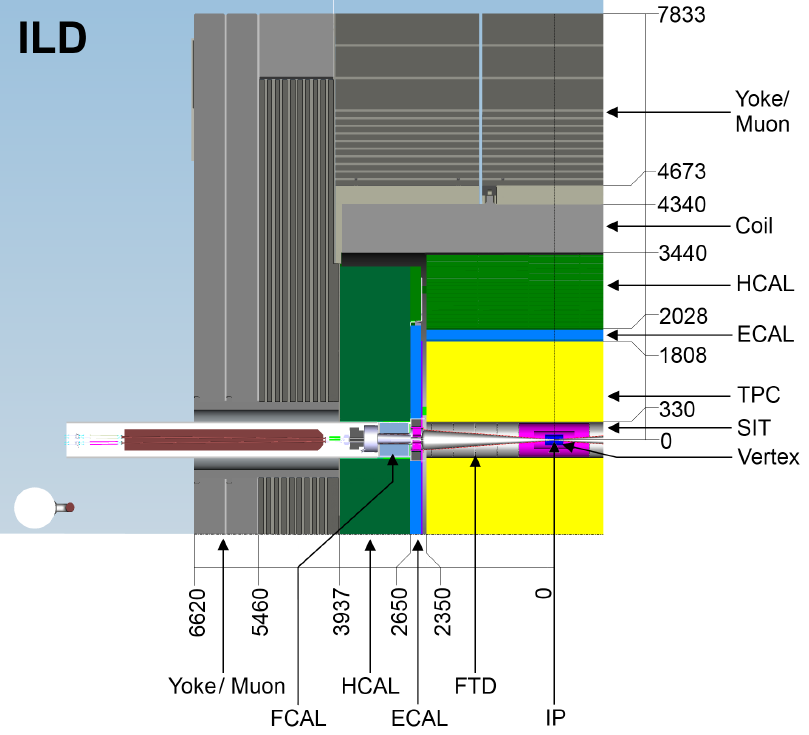
\includegraphics[width=0.75\textwidth]{../Pictures/ILDQuadrantView.png}
%	\caption{Quadrant view of the \acrshort{ILD} components.}
%	\label{figure:colliders/ILD/ILD-quadrant}
%\end{figure}
%
%% Image found here: https://flc.desy.de
%\begin{figure}[h]
%	\centering
%	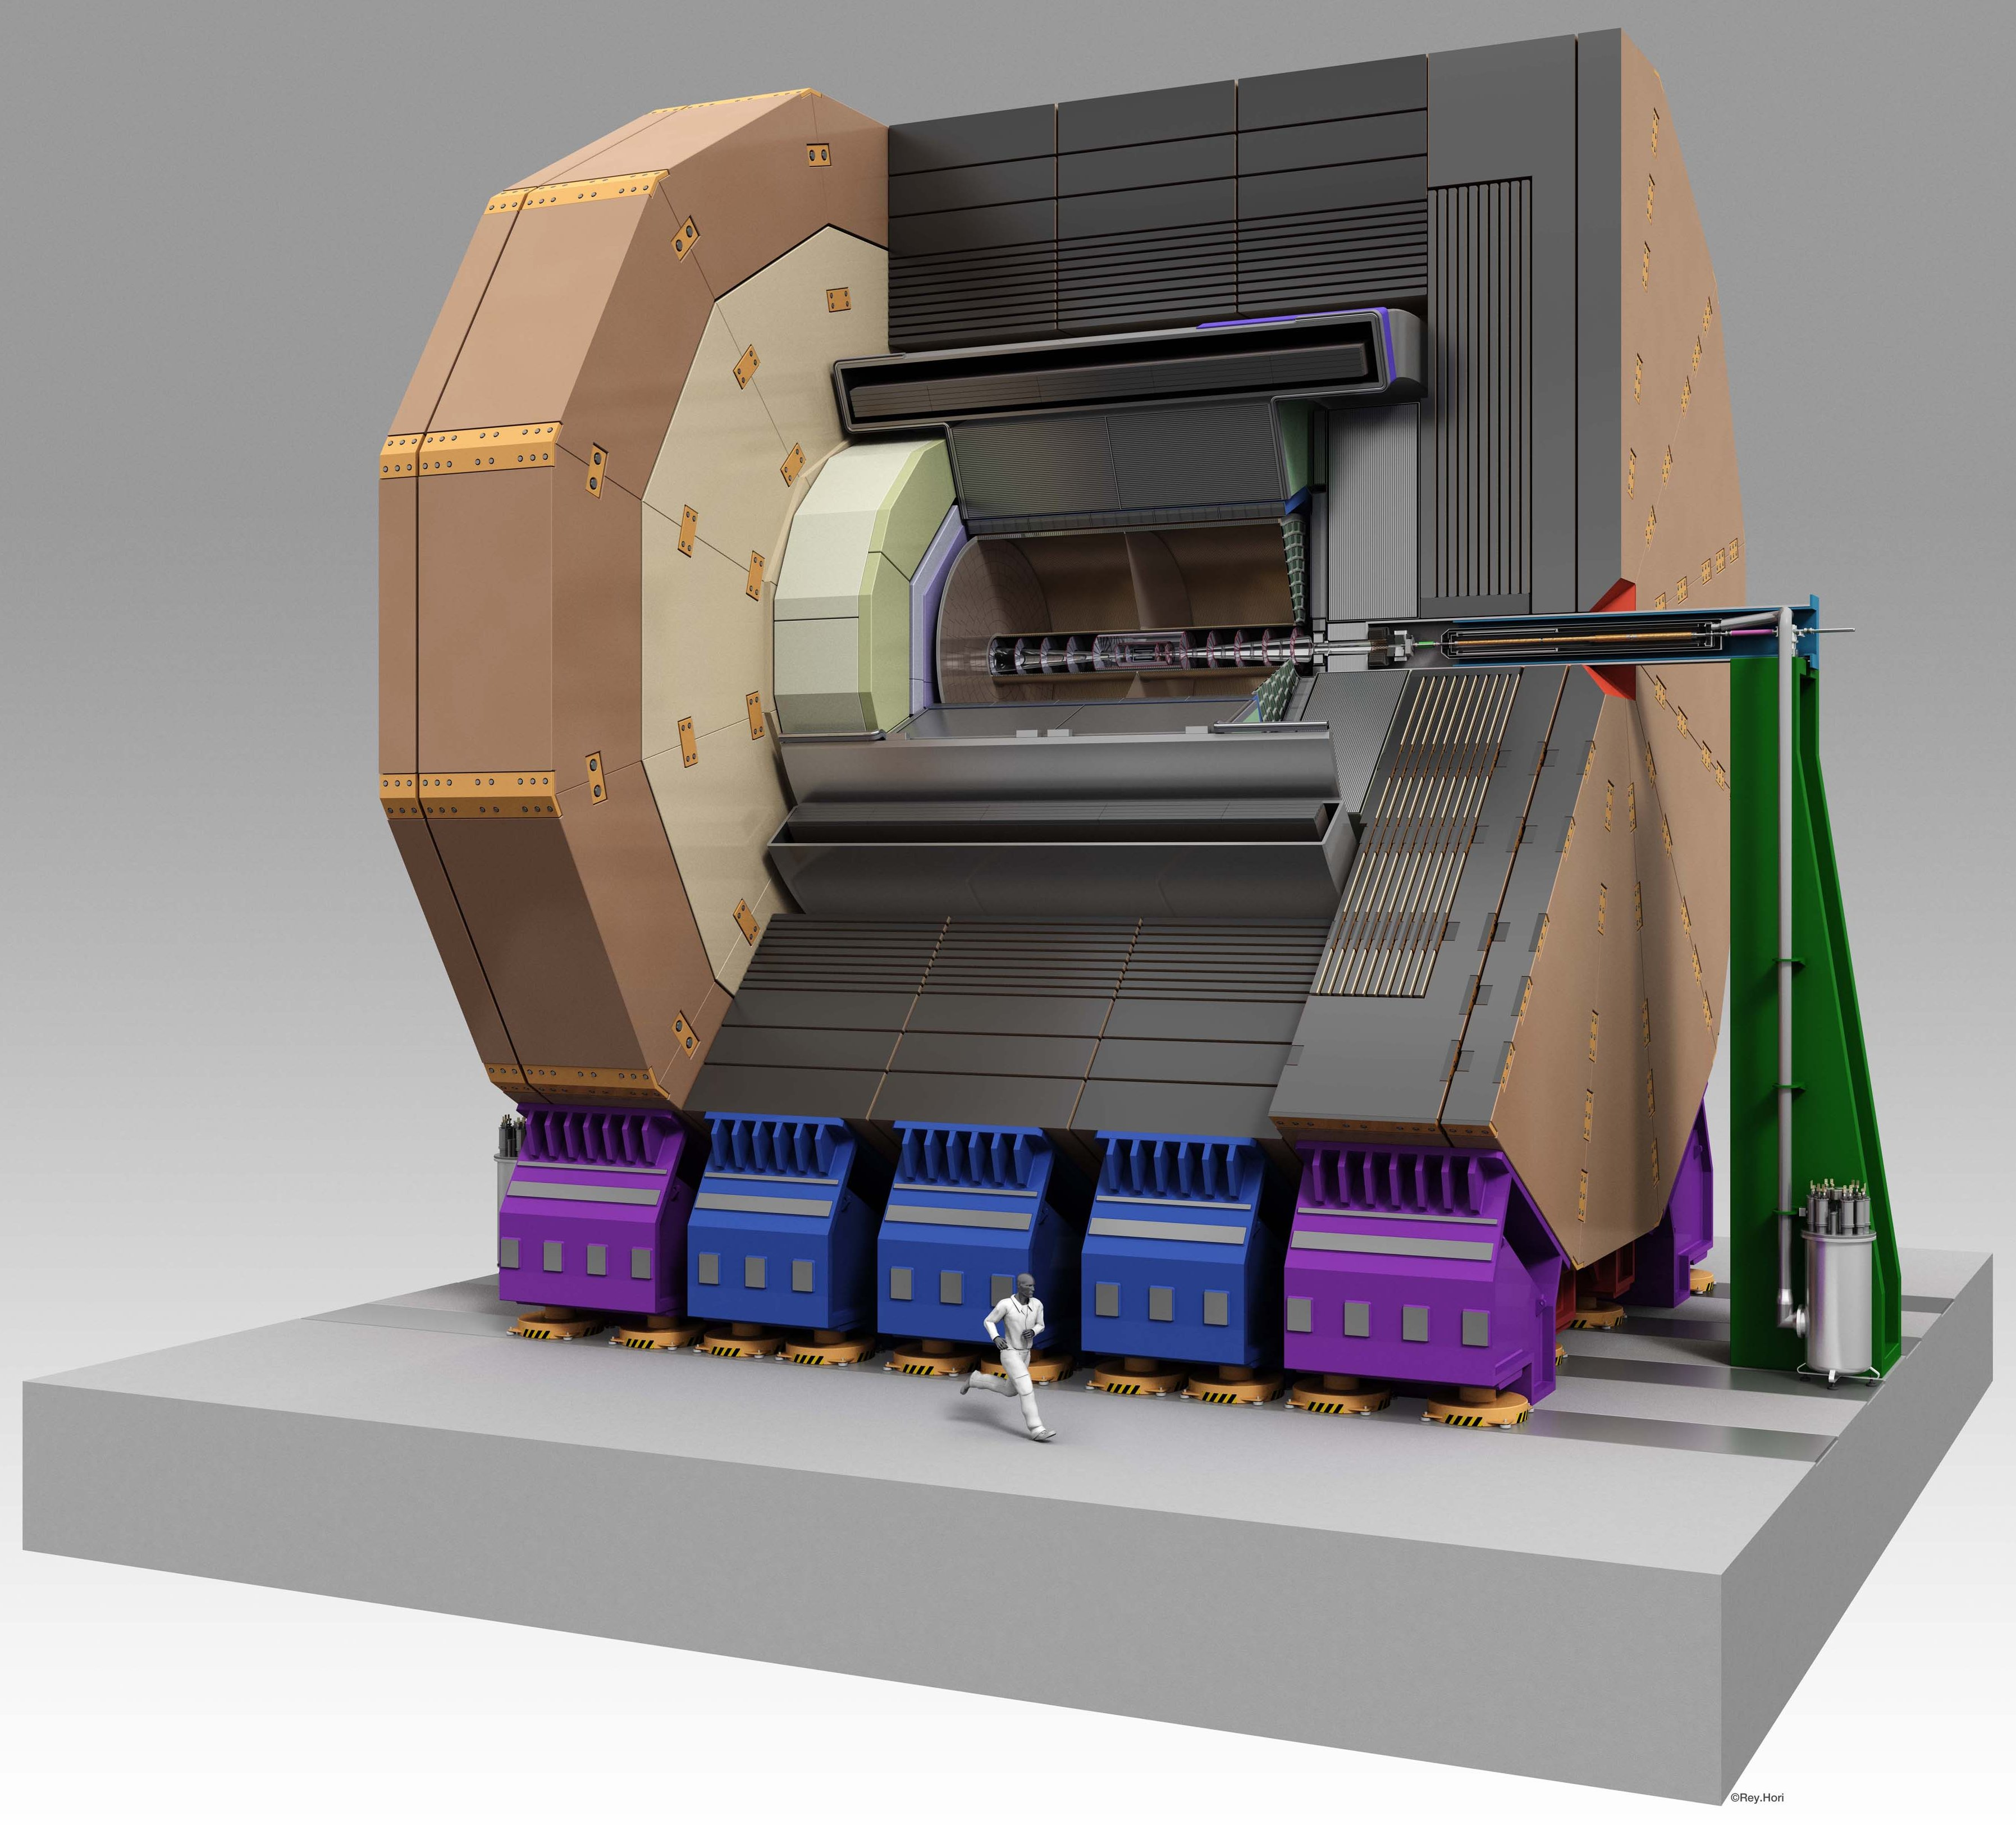
\includegraphics[width=0.75\textwidth]{../Pictures/ILDCutaway.jpg}
%	\caption{Rendering of the finished \acrshort{ILD}, cutaway to show the interal features, with human for scale.}
%	\label{figure:colliders/ILD/ILD-cutaway}
%\end{figure}

\begin{figure}[h]%
	\centering
    \subfloat{{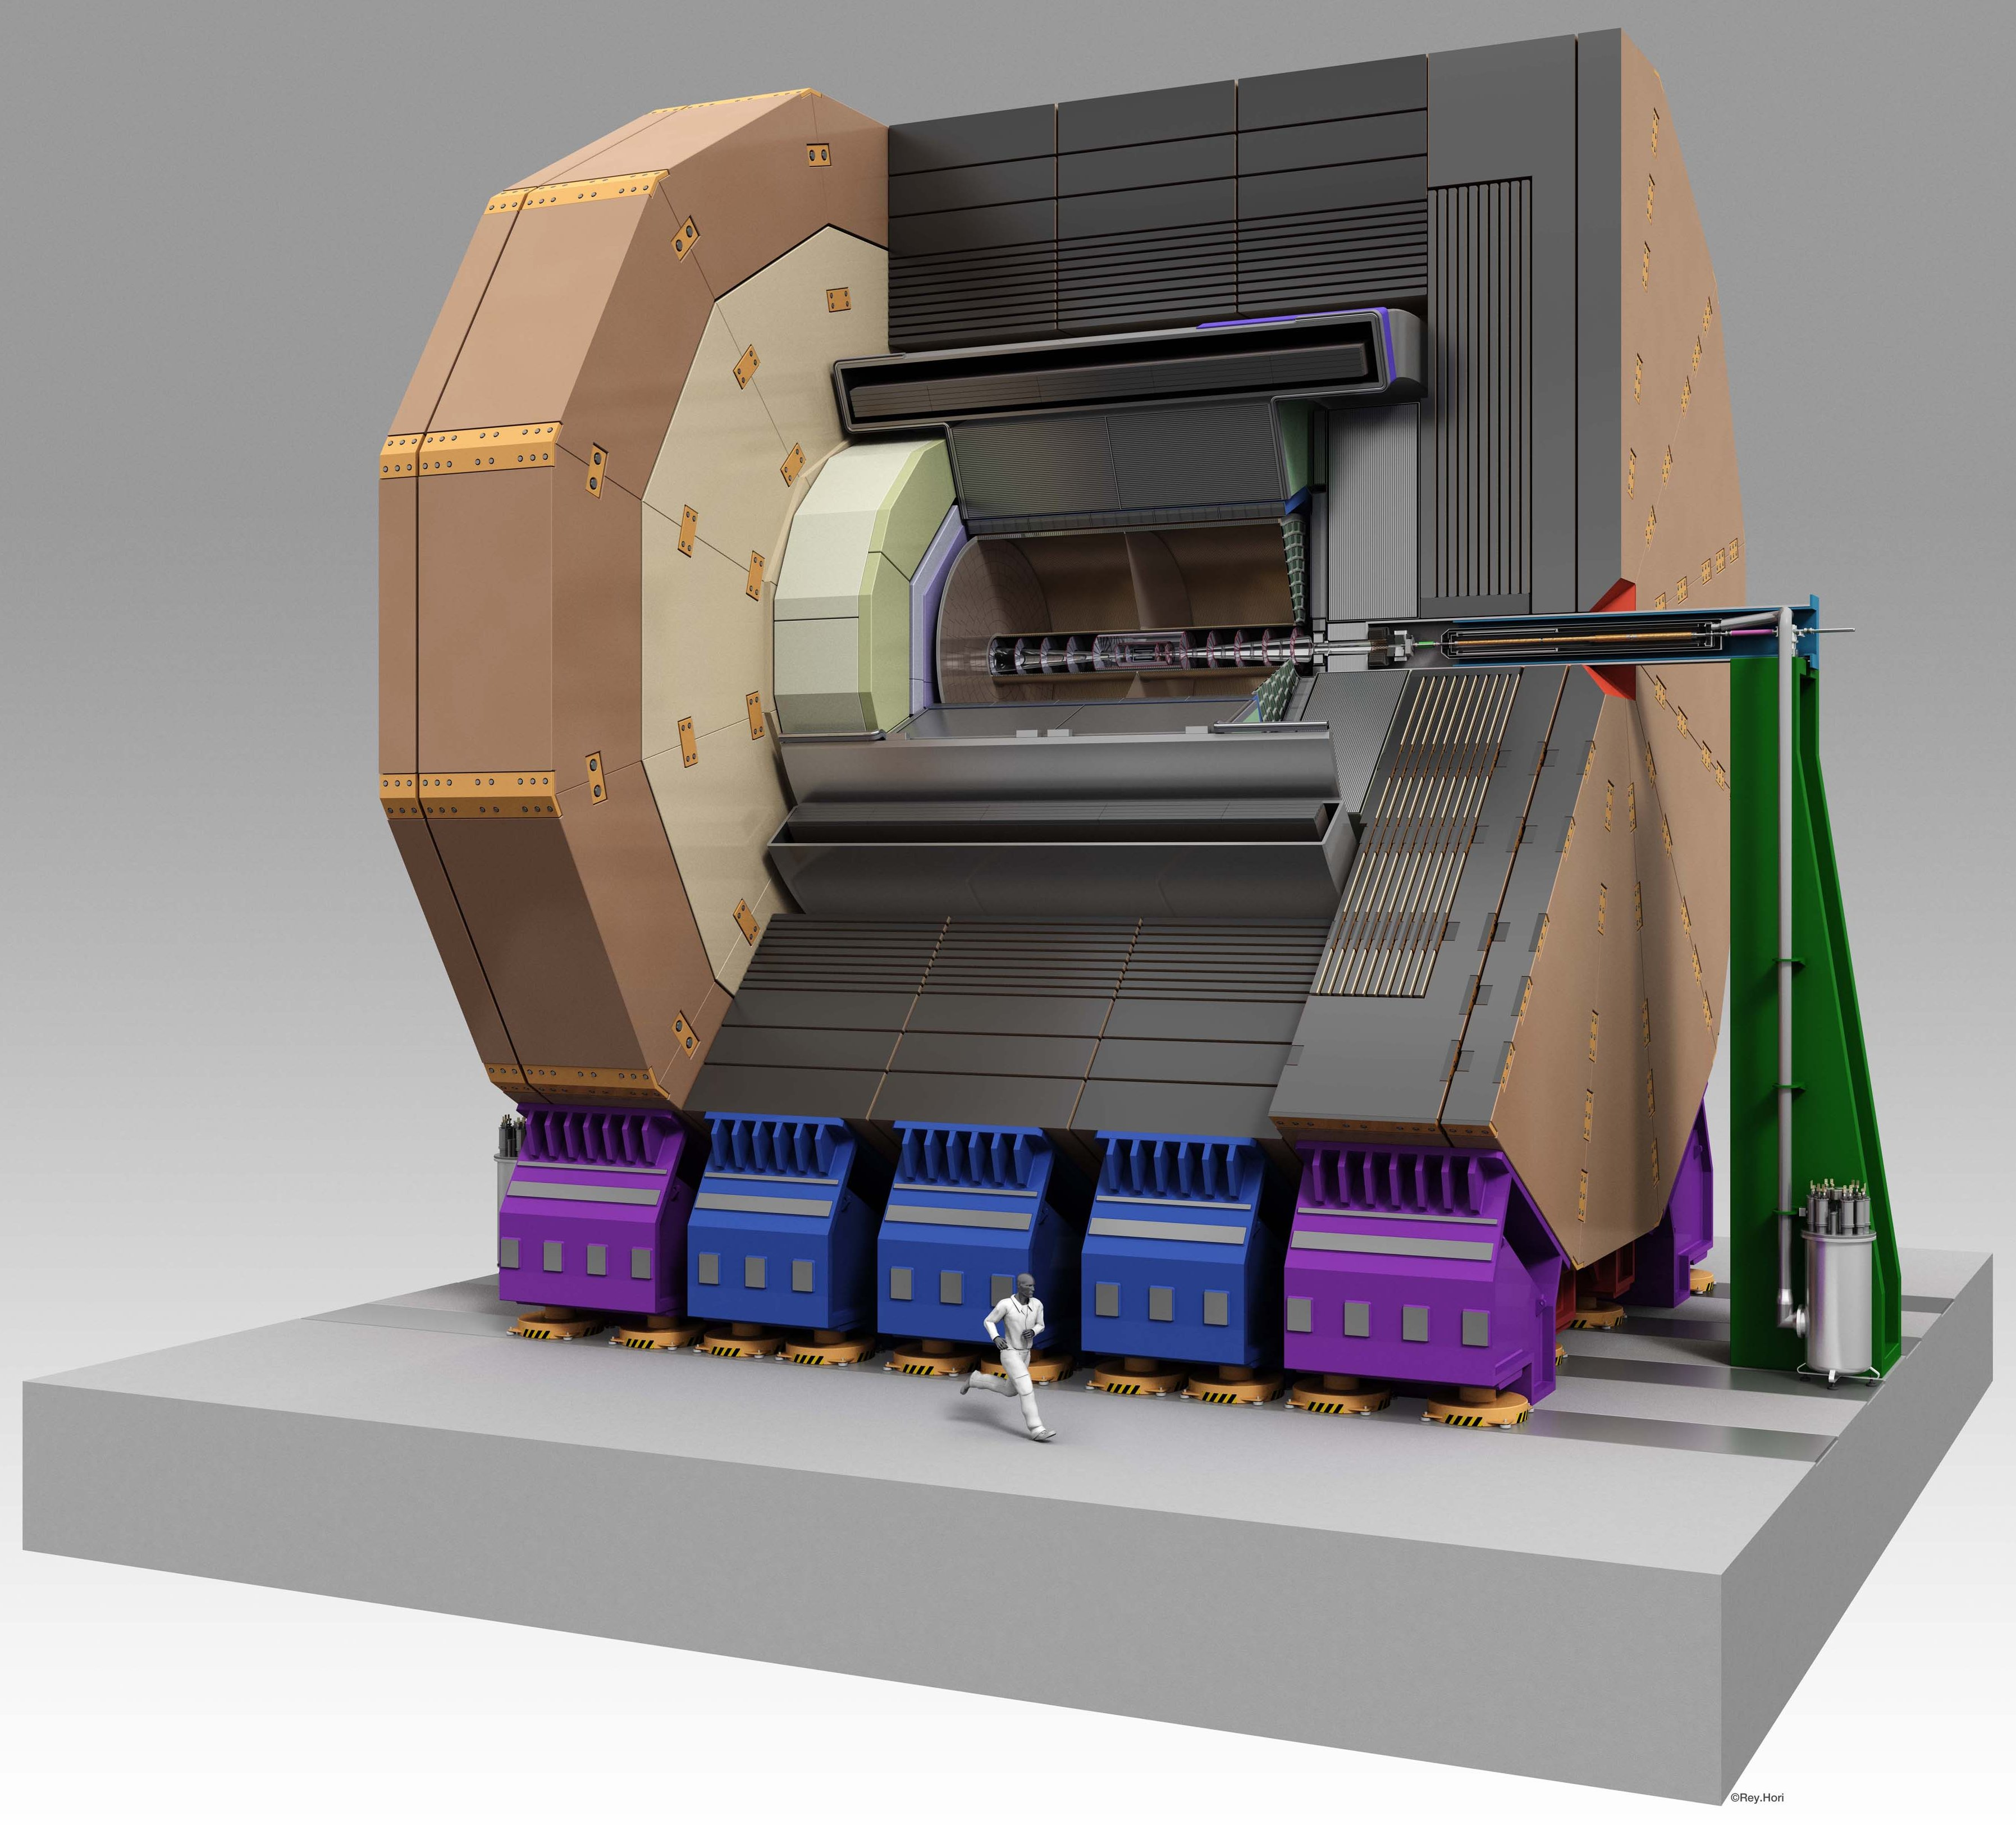
\includegraphics[width=0.45\textwidth]{../Pictures/ILDCutaway.jpg} }}%
    \qquad
	\subfloat{{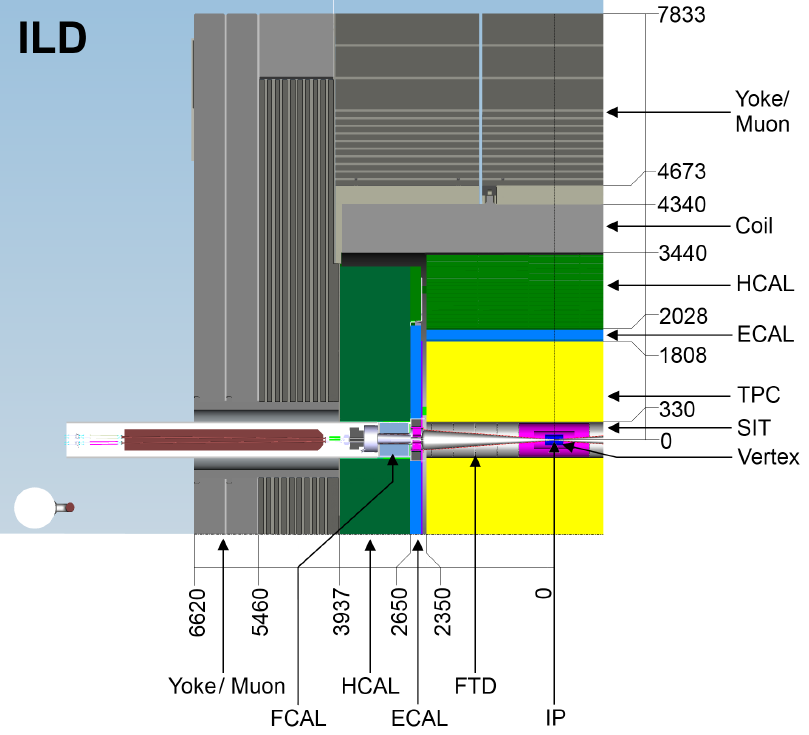
\includegraphics[width=0.45\textwidth]{../Pictures/ILDQuadrantView.png} }}%
    \caption{Rendering of the finished \acrshort{ILD} cutaway to show the interal features (left); and a quadrant view of the \acrshort{ILD} components (right).}%
    \label{figure:colliders/ILD/double}%
\end{figure}

\begin{figure}[h]
	\centering
	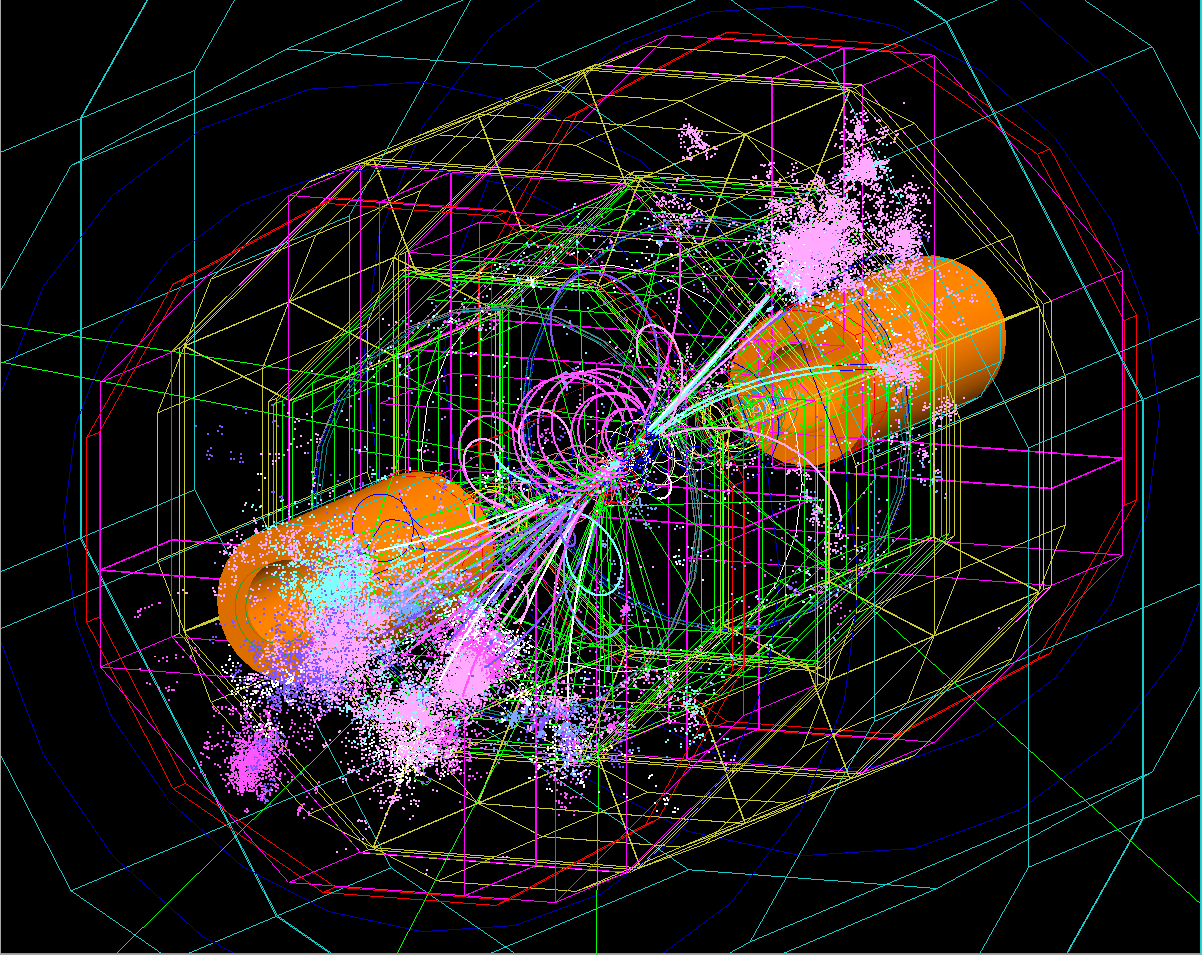
\includegraphics[width=0.75\textwidth]{../Pictures/SimulatedEvent1.png}
	\caption{Visualisation of a simulated $e^+ e^- \rightarrow t \overline{t} h$ event in the \acrshort{ILD}. Charged particles can be easily identified by the curved or spiral paths they take within the magnetic field, and the jets are visible as the light pink and purple areas near the beampipes on either side.}
	\label{figure:colliders/ILD/tth-simulation}
\end{figure}

\subsubsection{The Silicon Detector (SiD)}
The \acrfull{SiD} is a detector concept for the \acrshort{ILC} that uses primarily silicon-based technology, with the aim to reduce cost while still maintaining high performance and attaining the \acrshort{ILC}'s physics goals. The \acrshort{SiD} is also more compact than the \acrshort{ILD}, utilising a stronger magnetic field to compensate.

The vertex and tracker systems are both composed of silicon sensors, using a cylindrical configuration. The vertex uses silicon pixel sensors while the tracker uses silicon strip sensors, both designed to be used with power pulsing -- the electronics are only powered and active when it is known that bunches will be colliding. This reduces power and cooling requirements. 

The high-granularity calorimeters are both nested within the barrel, inside the magnetic field. The \acrshort{ECAL} uses thirty alternating layers of tungsten absorber and silicon active layers, in 3.5 $\times$ 3.5 mm\textsuperscript{2} hexagonal pixels. The \acrshort{HCAL} uses alternating layers of steel absorber and a glass resistive plate chamber, with cells of 10 $\times$ 10 mm\textsuperscript{2}

Outside of the calorimeter, the superconducting solenoid generates a 5T magnetic field, which enables the more compact detector design -- a higher magnetic field increases the spatial separation between charged and neutral particles, which is necessary for usage of particle flow algorithms.

Outside of the magnetic field is an iron flux return yoke, which similarly to the \acrshort{ILD} concept also acts as a strucutural support and is instrumented for muon identification and tail catching. 

\begin{figure}[h]%
	\centering
    \subfloat{{
\includegraphics[width=0.45\textwidth]{../Pictures/Placeholder.png} }}%
    \qquad
	\subfloat{{
\includegraphics[width=0.45\textwidth]{../Pictures/Placeholder.png} }}%
    \caption{Isometric view of the finished \acrshort{SiD} cutaway to show the interal features (left); and a quadrant view of the \acrshort{SiD} components (right).}%
    \label{figure:colliders/ILD/double}%
\end{figure}

\section{The Compact Linear Collider}
The \acrfull{CLIC} is a proposed linear electron-positron collider that [...]

[...]

The CLIC project foresees a programme spanning 22 years, over which multiple upgrades to the centre-of-mass energy would take place. Initial construction would be at 380 GeV, focusing on precision measurements of top-quark and Higgs physics. Further upgrades would increase the centre-of-mass energy to 1.5 TeV, then finally 3 GeV. Physics goals in these later stages would involve searches for new physics processes, as well as precision measurements of rare Higgs processes, and of new states discovered at the LHC or earlier stages of CLIC. 

[...] CLIC would be built beneath the existing LHC ring at CERN, stretching across the French-Swiss border and running parallel to the feet of the Jura mountain range. This placement is determined by the geological features of the region around Geneva and the feet of the Juras, [...]


[...]

As of writing, the CLIC project has been submitted as input for the European Particle Physics Strategy Update, which will decide which projects the CERN collaboration chooses to pursue from 2020  onwards. [...]

CLIC's initial centre-of-mass energy will be 380 GeV, with successive upgrades increasing this to 1.5 TeV and finally 3 TeV. 

The detecters envisoned for CLIC are similar in design to those for the ILC, and are usually referred to as CLIC\textunderscore ILD and CLIC\textunderscore SiD. [...] % Are the differences worth explaining?

\section{The Future Circular Collider}
The \acrfull{FCC} is a series of concepts for a future collider that would be located in the Geneva area near the existing LHC ring. The FCC project as a whole has three different accelerator concepts -- the FCC-hh for proton/proton and ion/ion collisions, the FCC-ee for electron/positron collisions, and the FCC-he for electron/proton collisions.

The initial proposal is to construct a circular electron/positron collider -- the FCC-ee -- with a circumference of 100km and delivering a maximum centre-of-mass energy of 365 GeV. The motivation for this is that at this energy range -- the electroweak scale -- the FCC would be able to access the Z pole, the W- and top-pair production thresholds, as well as producing a large number of Higgs bosons. 

A further part of the proposal for the FCC is that following the conclusion of the physics programme of the FCC-ee, the tunnels constructed to house the accelerator would be re-used for the FCC-hh, a hadron collider. This follows a similar use case as the LHC, which re-purposed the tunnels used for the \acrfull{LEP}. It is claimed that the FCC-hh built in these tunnels would be able to reach centre-of-mass energies of at least 100 TeV.

According to the given timeline, the FCC-ee would begin construction in 2028, and first physics would take place in 2039. 

%In general, the centre of mass energy of circular colliders is limited by losses to due synchrotron radiation. The energy loss per turn scales with $\frac{E^4}{m^4}$, meaning that lighter particles like electrons suffer more losses due to synchrotron radiation than heavier particles like hadrons. However, circular colliders provide significantly higher luminosities at energies in the 90-250 GeV range when compared to linear colliders. 

%FCC-ee physics:
%-Much higher luminosity beneath 400GeV
%-Multiple interaction points
%-Precision beam energy measurement through resonant transverse depolarisation
%-(Linear colliders have higher energy, easier longitudinal beam polarisation)
%-Large Higgs samples allows study of flavour-violating Higgs and very rare SM decays

[...]

\section{The Circular Electron Positron Collider}

The \acrfull{CEPC} is a proposal for a circular electron-positron collider 

[...]